\documentclass[11pt]{article}

\usepackage[margin=1in]{geometry}
\usepackage{amsmath,amssymb,amsthm}
\usepackage{booktabs}
\usepackage{graphicx}
\usepackage{subcaption}
\usepackage[round,authoryear]{natbib}
\usepackage[colorlinks=true,citecolor=blue,linkcolor=blue]{hyperref}

\newcommand{\iid}{\mathrel{\overset{\mathrm{iid}}{\sim}}}
\DeclareMathOperator{\Var}{Var}
\DeclareMathOperator{\E}{E}

\newtheorem{theorem}{Theorem}
\theoremstyle{definition}
\newtheorem{definition}{Definition}

\title{STAT 5014 Homework 1}
\author{Junru Yao}
\date{August 25, 2026}

\begin{document}

\maketitle

\section{Setup and definitions}

Let $X_1,\ldots,X_n \iid F$ with $\E[X_i]=\mu$ and
$\Var(X_i)=\sigma^2<\infty$. The sample mean and sample variance are
\[
  \bar X_n=\frac{1}{n}\sum_{i=1}^n X_i
  \qquad\text{and}\qquad
  S^2=\frac{1}{n-1}\sum_{i=1}^n (X_i-\bar X_n)^2.
\]

\begin{definition}
An estimator $\hat\theta$ is \emph{unbiased} for $\theta$ if
$\E[\hat\theta]=\theta$ for every $\theta$ in the parameter space.
\end{definition}

\section{A short derivation}

The variance of a random variable $X$ with mean $\mu$ can be rewritten as
\begin{equation}
  \Var(X)=\E[X^2]-\mu^2.
  \label{eq:variance}
\end{equation}
To see this, expand the definition:
\begin{align}
  \Var(X) &= \E\big[(X-\mu)^2\big] \\
           &= \E\big[X^2-2\mu X+\mu^2\big] \\
           &= \E[X^2]-2\mu\E[X]+\mu^2 \\
           &= \E[X^2]-\mu^2,
\end{align}
which is Equation~\eqref{eq:variance}.

\section{A theorem}

\begin{theorem}[Central Limit Theorem]
Let $X_1,\ldots,X_n \iid F$ with mean $\mu$ and finite variance
$\sigma^2>0$. Then
\[
  \sqrt{n}(\bar X_n-\mu)\xrightarrow{d}\mathcal{N}(0,\sigma^2)
  \qquad\text{as }n\to\infty.
\]
\end{theorem}

\begin{proof}
Omitted; see \citet[Ch.~5]{casella2002}.
\end{proof}

Note that Theorem~1 requires only finite variance, not normality of $F$.

\section{Matrices and piecewise functions}

Let $(Y_1,Y_2)^\top$ be bivariate normal with correlation $\rho$ and
marginal standard deviations $\sigma_1$ and $\sigma_2$. Its covariance
matrix is
\[
  \Sigma=
  \begin{pmatrix}
    \sigma_1^2 & \rho\,\sigma_1\sigma_2 \\
    \rho\,\sigma_1\sigma_2 & \sigma_2^2
  \end{pmatrix},
  \qquad \rho\in[-1,1].
\]
The indicator function of the event $\{X>0\}$ is
\[
  \mathbf{1}\{X>0\}=
  \begin{cases}
    1 & \text{if }X>0,\\
    0 & \text{otherwise.}
  \end{cases}
\]

\section{A small simulation study}

Suppose we simulate data from the model
\begin{equation}
  y_i=\beta_0+\beta_1x_i+\varepsilon_i,
  \qquad \varepsilon_i\iid\mathcal{N}(0,\sigma^2),
  \label{eq:model}
\end{equation}
and estimate $\beta$ by ordinary least squares,
$\hat\beta=(X^\top X)^{-1}X^\top y$. The settings are given in
Table~\ref{tab:settings}, and the fit for the baseline scenario appears in
Figure~\ref{fig:simulation}.

\begin{table}[htbp]
  \centering
  \caption{Settings for the simulation study.}
  \label{tab:settings}
  \begin{tabular}{lrrr}
    \toprule
    Scenario & Sample size $n$ & Noise SD $\sigma$ & Replicates \\
    \midrule
    Baseline & 60  & 1.0 & 1000 \\
    Larger   & 200 & 1.0 & 1000 \\
    Noisier  & 60  & 2.5 & 1000 \\
    \bottomrule
  \end{tabular}
\end{table}

\begin{figure}[htbp]
  \centering
  \begin{subfigure}[t]{0.48\textwidth}
    \centering
    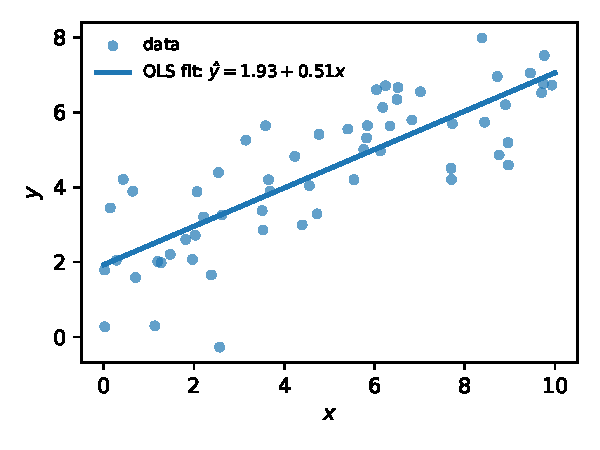
\includegraphics[width=\linewidth]{figures/scatter.pdf}
    \caption{Fitted model.}
    \label{fig:scatter}
  \end{subfigure}\hfill
  \begin{subfigure}[t]{0.48\textwidth}
    \centering
    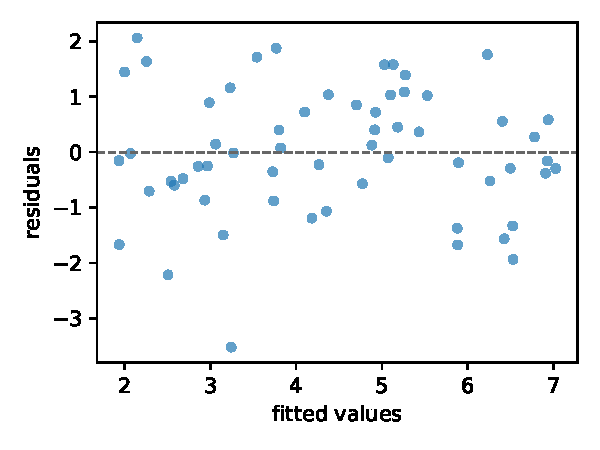
\includegraphics[width=\linewidth]{figures/residuals.pdf}
    \caption{Residual diagnostic.}
    \label{fig:residuals}
  \end{subfigure}
  \caption{Simulated data from Equation~\eqref{eq:model} with an ordinary
  least-squares fit. Panel~\subref{fig:residuals} shows no obvious departure
  from the constant-variance assumption.}
  \label{fig:simulation}
\end{figure}

Uncertainty in $\hat\beta$ could also be assessed without distributional
assumptions by resampling \citep{efron1979}, and a penalized alternative is
available when $p$ is large \citep{tibshirani1996}. I am also interested in
ensemble learning, for which random forests provide a flexible approach to
classification and regression \citep{breiman2001}.

\bibliographystyle{plainnat}
\bibliography{hw1}

\end{document}
